\documentclass[aspectratio=169,11pt]{beamer}
\def\courseweek{3}
% Shared style for the Introduction to Information Geometry lecture slides.
% Compile the lecture .tex files from this directory.
\providecommand{\courseweek}{1}
\usepackage[T1]{fontenc}
\usepackage[utf8]{inputenc}
\usepackage[sc]{mathpazo}
\renewcommand{\sfdefault}{lmss}
\renewcommand{\ttdefault}{lmtt}
\usepackage{amsmath,amssymb,mathtools}
\usepackage{tikz}
\usetikzlibrary{arrows.meta,calc,positioning}
\usepackage{pgfplots}
\pgfplotsset{compat=1.18}
\usepackage{booktabs}

\definecolor{courseink}{HTML}{173749}
\definecolor{coursemuted}{HTML}{526674}
\definecolor{courseteal}{HTML}{0E7287}
\definecolor{coursecopper}{HTML}{B66B43}
\definecolor{courseline}{HTML}{D4E0E3}
\definecolor{coursepale}{HTML}{EFF5F5}

\setbeamercolor{normal text}{fg=courseink,bg=white}
\setbeamercolor{structure}{fg=courseteal}
\setbeamercolor{frametitle}{fg=courseink,bg=white}
\setbeamercolor{title}{fg=courseink}
\setbeamercolor{subtitle}{fg=coursemuted}
\setbeamercolor{block title}{fg=courseink,bg=white}
\setbeamercolor{block body}{fg=courseink,bg=white}
\setbeamercolor{alerted text}{fg=coursecopper}
\setbeamerfont{title}{family=\rmfamily,series=\bfseries,size=\fontsize{32}{37}}
\setbeamerfont{frametitle}{family=\rmfamily,series=\bfseries,size=\fontsize{26}{31}}
\setbeamerfont{normal text}{size=\fontsize{18}{22}}
\setbeamerfont{subtitle}{size=\fontsize{17}{21}}
\setbeamersize{text margin left=0.78cm,text margin right=0.78cm}
\setbeamertemplate{navigation symbols}{}
\setbeamertemplate{itemize items}[circle]
\setbeamertemplate{enumerate items}[default]
\setbeamertemplate{blocks}[default]
\setlength{\parskip}{0.22em}
\setbeamertemplate{footline}{%
  \leavevmode\hbox to \paperwidth{\hspace{.78cm}%
  {\color{coursemuted}\fontsize{8.5}{10}\selectfont Introduction to Information Geometry \hspace{.32cm} / \hspace{.32cm} Week \courseweek}%
  \hfill{\color{coursemuted}\fontsize{8.5}{10}\selectfont \insertframenumber\hspace{.17cm}/\hspace{.17cm}\inserttotalframenumber}\hspace{.78cm}}%
  \vskip.17cm
}
\setbeamertemplate{frametitle}{%
  \vspace{.13cm}
  \insertframetitle\par
  \vspace{.08cm}
}
\setbeamertemplate{title page}{%
  \vspace*{1.00cm}
  {\color{courseteal}\fontsize{10}{13}\selectfont\bfseries
  INTRODUCTION TO INFORMATION GEOMETRY\par}
  \vspace{.40cm}
  {\usebeamerfont{title}\usebeamercolor[fg]{title}\inserttitle\par}
  \vspace{.22cm}
  {\usebeamerfont{subtitle}\usebeamercolor[fg]{subtitle}\insertsubtitle\par}
  \vfill
  {\color{coursemuted}\fontsize{13}{16}\selectfont Christopher Lee\par}
  \vspace{.34cm}
}

\pgfplotsset{
  courseplot/.style={
    width=11.05cm,
    height=5.15cm,
    axis line style={coursemuted!75},
    tick style={coursemuted!65},
    ticklabel style={font=\scriptsize,color=coursemuted},
    label style={font=\normalsize,color=courseink},
    grid=major,
    major grid style={courseline!70,line width=.4pt},
    line width=1.45pt,
    legend style={font=\small,draw=none,fill=none,at={(.98,.03)},anchor=south east},
    clip=true
  }
}

\newcommand{\highlightmath}[1]{{\color{courseteal}#1}}
\newcommand{\thinrule}{\par\vspace{.25cm}{\color{courseline}\rule{\linewidth}{.8pt}}\par}

% A one-dimensional state space.  x=0 and x=1 are placed at 0 and 9 units.
\newcommand{\stateinterval}[1]{%
 \begin{tikzpicture}[x=1cm,y=1cm]
   \draw[courseink,line width=1.25pt] (0,0)--(9,0);
   \foreach \pos/\lab in {0/0,9/1} {
     \fill[courseink] (\pos,0) circle(2.7pt);
     \node[below=9pt,text=coursemuted] at (\pos,0) {\(\lab\)};
   }
   #1
 \end{tikzpicture}%
}

% Paired pages are separate frames in the PDF, with matching titles.
% Supply the whole frame body for each version; the instructor may edit them
% independently without changing overlay logic.
\newcommand{\coursepair}[3]{%
  \begin{frame}{#1}#2\end{frame}%
  \begin{frame}{#1}#3\end{frame}%
}

% Equilateral representation of the categorical simplex, in barycentric
% coordinates with vertices A=(0,0), B=(1,0), C=(1/2,sqrt(3)/2).
\newcommand{\coursesimplex}[1]{%
 \begin{tikzpicture}[scale=4.9]
  \fill[coursepale] (0,0)--(1,0)--(.5,.8660254)--cycle;
  \draw[courseink,line width=.65pt] (0,0)--(1,0)--(.5,.8660254)--cycle;
  \node[below left,font=\small] at (0,0) {A};
  \node[below right,font=\small] at (1,0) {B};
  \node[above,font=\small] at (.5,.8660254) {C};
  #1
 \end{tikzpicture}%
}

\title{Cyclic Motion and Invasion}
\subtitle{Week 3 \(\cdot\) Lecture 2}
\date{}
\begin{document}
\begin{frame}[plain]\titlepage\end{frame}

\begin{frame}{One family, three kinds of motion}
For
\[
M_s=\begin{pmatrix}0&1&-s\\-s&0&1\\1&-s&0\end{pmatrix},
\qquad s>0,
\]
the equal mixture \(\mathbf p^*=(\frac13,\frac13,\frac13)\) is an equilibrium.
\vspace{.5cm}
As \(s\) varies, trajectories may approach the center, remain on
closed curves, or move toward the boundary.
\end{frame}

\begin{frame}{A scalar quantity for cyclic motion}
For an interior population set
\[
P=p_Ap_Bp_C,\qquad
Q=p_Ap_B+p_Bp_C+p_Cp_A.
\]
\vspace{.4cm}
The product satisfies
\[
0<P\leq\frac1{27},
\]
\vspace{.26cm}
with equality only at the equal mixture.
\vspace{.34cm}
The motion of \(P\) detects movement toward or away from the center.
\end{frame}

\coursepair{Differentiating the product}{
Take \(P=p_Ap_Bp_C>0\). Differentiate the logarithm:
\[
\frac{d}{dt}\ln P=\sum_i\frac{p_i'}{p_i}=\sum_i(f_i-\bar f).
\]
\vspace{.35cm}
For the cyclic family, \(\sum_i f_i=1-s\) and \(\bar f=(1-s)Q\).
Find \(\frac{d}{dt}\ln P\).
}{
Take \(P=p_Ap_Bp_C>0\). Differentiate the logarithm:
\[
\frac{d}{dt}\ln P=\sum_i\frac{p_i'}{p_i}=\sum_i(f_i-\bar f).
\]
\vspace{.35cm}
Using \(\sum_i f_i=1-s\) and \(\bar f=(1-s)Q\),
\[
\highlightmath{\frac{d}{dt}\ln P=(1-s)(1-3Q)}.
\]
}

\begin{frame}{The second factor is nonnegative}
Because \(p_A+p_B+p_C=1\),
\[
\highlightmath{1-3Q=\frac12\Bigl[(p_A-p_B)^2+(p_B-p_C)^2
 +(p_C-p_A)^2\Bigr]}.
\]
\vspace{.5cm}
Thus \(1-3Q>0\) away from the equal mixture.
\vspace{.4cm}
The sign of \(\frac{d}{dt}\ln P\) is controlled by \(1-s\).
\end{frame}

\begin{frame}{Three regimes around the center}
\begin{center}
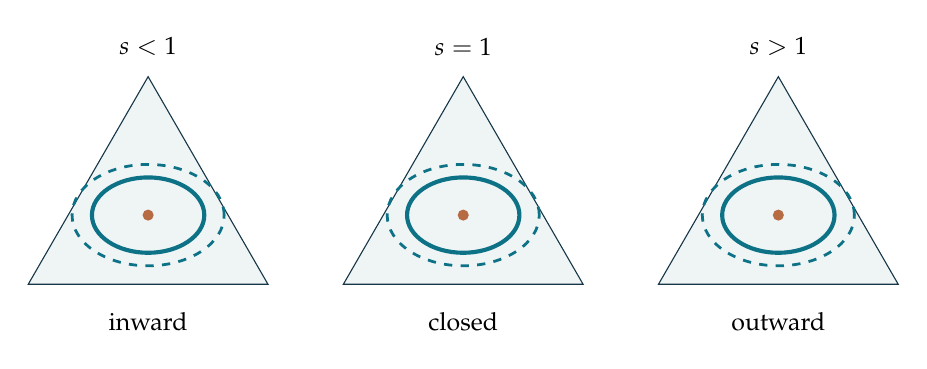
\begin{tikzpicture}[scale=.87]
\foreach \xx/\ss/\note in {0/{s<1}/{inward},4.6/{s=1}/{closed},9.2/{s>1}/{outward}}{
 \begin{scope}[xshift=\xx cm]
 \fill[coursepale](0,0)--(3.5,0)--(1.75,3.031)--cycle;
 \draw[courseink](0,0)--(3.5,0)--(1.75,3.031)--cycle;
 \fill[coursecopper](1.75,1.01)circle(2.3pt);
 \node[above,font=\small]at(1.75,3.2){\(\ss\)};
 \node[below,font=\small]at(1.75,-.27){\note};
 \draw[courseteal,line width=1.5pt] (1.75,1.01)ellipse[x radius=.82,y radius=.55];
 \draw[courseteal,line width=1pt,dashed] (1.75,1.01)ellipse[x radius=1.11,y radius=.74];
 \end{scope}
}
\end{tikzpicture}
\end{center}
\vspace{.10cm}
The ellipses schematically show nested product levels.
\end{frame}

\begin{frame}{What the product proves}
\begin{itemize}\setlength{\itemsep}{.6cm}
\item \(s<1\): \(P\) increases toward its maximum \(1/27\). Interior motion approaches the center.
\item \(s=1\): \(P\) is conserved. Noncentral interior solutions are periodic.
\item \(s>1\): \(P\) decreases toward zero. Interior motion approaches the boundary as a set.
\end{itemize}
\end{frame}

\begin{frame}{Linearizing the cyclic system}
Use \(x=p_A\), \(y=p_B\), and \(p_C=1-x-y\).
\vspace{.4cm}
At the center, the Jacobian is
\[
\highlightmath{J_s=\frac13\begin{pmatrix}s&s+1\\-(s+1)&-1\end{pmatrix}}.
\]
\vspace{.35cm}
Its eigenvalues are
\[
\lambda_\pm=\frac{s-1}{6}\pm i\frac{\sqrt3(s+1)}6.
\]
\end{frame}

\coursepair{A damped cycle}{
Take \(s=0.7\). From
\[
\lambda_\pm=\frac{s-1}{6}\pm i\frac{\sqrt3(s+1)}6,
\]
\vspace{.30cm}
find the decay rate \(\rho\), angular frequency \(\omega\), and
approximate small-oscillation period \(T=2\pi/\omega\).
}{
Take \(s=0.7\). The eigenvalues have
\[
\highlightmath{\rho=-0.05},\qquad
\highlightmath{\omega\approx0.491}.
\]
\vspace{.30cm}
The small-oscillation period is
\[
\highlightmath{T=\frac{2\pi}{\omega}\approx12.80}.
\]
\vspace{.26cm}
The linear envelope decays like \(e^{-0.05t}\).
}

\begin{frame}{Stability within a face}
A population on the AB edge can attract all other states of that edge.
\vspace{.46cm}
To assess stability in the full triangle, we must also ask whether
a small number of C individuals can grow.
\vspace{.40cm}
At a face equilibrium \(q\), the initial growth of a missing type is
\[
\highlightmath{p_C'\approx p_C\big(f_C(q)-\bar f(q)\big)}.
\]
\end{frame}

\coursepair{An invader changes the stability question}{
Let
\[
M=\begin{pmatrix}0&2&0\\2&0&0\\3&3&0\end{pmatrix},
\qquad q=(\tfrac12,\tfrac12,0).
\]
\vspace{.33cm}
At \(q\), find \(\bar f\) and C's invasion rate
\(f_C(q)-\bar f(q)\).
}{
Let
\[
M=\begin{pmatrix}0&2&0\\2&0&0\\3&3&0\end{pmatrix},
\qquad q=(\tfrac12,\tfrac12,0).
\]
\vspace{.33cm}
The fitnesses at \(q\) are \((1,1,3)\), hence \(\bar f=1\).
\[
\highlightmath{f_C(q)-\bar f(q)=3-1=2>0}.
\]
}

\begin{frame}{An invariant edge may be unstable in the triangle}
At \(q=(\frac12,\frac12,0)\), the AB-edge equation is
\[
x'=x(1-x)(2-4x).
\]
\vspace{.43cm}
Its derivative at \(x=\frac12\) is \(-1\): attraction along the edge.
\vspace{.4cm}
But a small C introduction has \(p_C'\approx2p_C\),
so \(q\) repels in that transverse direction.
\end{frame}

\begin{frame}{From populations to probability laws}
Every normalized vector is a categorical distribution.
\vspace{.4cm}
\[
\highlightmath{\mathbf p(t)=(p_A(t),p_B(t),p_C(t))}.
\]
\vspace{.4cm}
The simplex is simultaneously a state space for a dynamical system
and a space of possible sampling probabilities.
\vspace{.4cm}
Next week, we study that probability interpretation directly.
\end{frame}
\end{document}
